\section{Training}
\label{training_detail}

MiniOneRec first converts item text into discrete codes. Titles and descriptions are embedded by the Qwen3-Embedding-4B encoder, after which RQ-VAE performs residual quantization. This tokenizer is trained on a single GPU with a batch size of 20\,480, a learning rate of $1\times10^{-3}$, and 10,000 training epochs. The resulting SID vocabulary is plugged into a Qwen2.5-Instruct backbone. SFT takes place on eight NVIDIA H100, each holding 128 samples. Training lasts up to ten epochs with early stopping (patience one epoch). The initial learning rate is $3\times10^{-4}$ and follows a cosine decay schedule. Starting from the SFT checkpoint, we apply GRPO for two additional epochs while keeping the KL weight $\beta$ unchanged. During roll-out, beam search with width 16 is adopted, so every input generates sixteen distinct candidate sequences.

In the performance comparison with existing recommenders, conventional recommenders are trained with binary cross-entropy and the Adam optimizer; learning rates are chosen from \{1e-2, 1e-3, 1e-4\}, and the weight-decay term is scanned over \{1e-2, 1e-3, 1e-4, 1e-5, 1e-6\}. The batch size is 1\,024.  
For TIGER, we rely on a T5 encoder–decoder and reuse Qwen3-Embedding-4B for item embeddings.  
All LLM-powered systems, including ours, share the Qwen2.5-Instruct backbone and use AdamW. Batches contain 128 examples for SFT and preference alignment, and 512 samples for RL. The learning rate is $3\times10^{-4}$ during SFT, while S-DPO and RL use $1\times10^{-5}$. S-DPO runs for one epoch with $\beta=0.1$ and samples three negative items; D$^{3}$ tries interpolation factors $\alpha$ of 0.8, 0.9, and 1.0.

\section{Evaluation}
\label{results}

This section details our empirical study. We begin with a scaling investigation on two real-world benchmarks \citep{amazon}, examining how MiniOneRec’s loss curves change as model size grows. We then benchmark MiniOneRec against three groups of baselines: traditional sequential recommenders, SID-based generators, and recent LLM-driven systems.  
To evaluate the model’s capability for cross-domain recommendation generalization, we frame SID next-item prediction as a task of recommendation rule discovery and evaluate the model on domains that never appeared during training.  
Comprehensive ablation tests follow, which help us locate the parts of the framework that contribute most to the final score. Finally, we look into how the broad knowledge stored in pre-trained LLM weights affects generative recommendation.
In summary, we study the following questions within this section:

\begin{itemize}
    \item How does the loss of MiniOneRec scale with different model size?
    
    \item How does MiniOneRec perform in comparison to other baseline methods?
    
    \item How does MiniOneRec perform under completely unseen domains?
    
    \item How do the designed components contribute to MiniOneRec's recommendation efficiency?

    \item How do the pre-trained weights of the LLM influence the performance of generative recommendation?
    % What is the impact of the designed components on the recommendation performance of MiniOneRec?

\end{itemize}

\subsection{Evaluation Setup}

% \textbf{Datasets and Metrics.} 

Experiments are carried out on two real-world slices of the Amazon Review dataset \citep{amazon}, namely \textit{Office} and \textit{Industrial}. To measure top-$K$ recommendation accuracy, we follow standard practice and compute Hit Rate (HR@K) as well as Normalized Discounted Cumulative Gain (NDCG@K).


% Please add the following required packages to your document preamble:
% \usepackage{multirow}
\begin{table}[t]
\caption{Performance of MiniOneRec Compared to Traditional Methods, Generative Methods, and LLM-based Methods} 
\label{tab:overall}
\centering
\begin{adjustbox}{max width=0.9\textwidth}
\renewcommand{\arraystretch}{1.00}
% \begin{tabular}{clllllll}
\begin{tabular}{cccccccc}
\toprule
\multicolumn{1}{c}{Datasets}            & Methods    & HR@3   & NDCG@3 & HR@5   & NDCG@5 & HR@10  & NDCG@10 \\ \midrule
% \multicolumn{1}{l}{Datesets}           & Methods    & HR@3   & NDCG@3 & HR@5   & NDCG@5 & HR@10  & NDCG@10 \\ \midrule
\multirow{14}{*}{\textbf{Industrial}} & \multicolumn{7}{c}{\textbf{Traditional}}                          \\ \cmidrule(lr){2-8} 
                                      & GRU4Rec    & 0.0638 & 0.0542 & 0.0774 & 0.0598 & 0.0999 & 0.0669  \\
                                      & Caser      & 0.0618 & 0.0514 & 0.0717 & 0.0555 & 0.0942 & 0.0628  \\
                                      & SASRec     & 0.0790 & 0.0700 & 0.0909 & 0.0748 & 0.1088 & 0.0806  \\ \cmidrule(lr){2-8}
                                      & \multicolumn{7}{c}{\textbf{Generative}}                           \\ \cmidrule(lr){2-8}
                                      & HSTU       & 0.0927 & 0.0885 & 0.1037 & 0.0918 & 0.1163 & 0.0958  \\
                                      & TIGER      & 0.0852 & 0.0742 & 0.1010 & 0.0807 & 0.1321 & 0.0908  \\
                                      & LCRec      & 0.0915 & 0.0805 & 0.1057 & 0.0862 & 0.1332 & 0.0952  \\ \cmidrule(lr){2-8}
                                      & \multicolumn{7}{c}{\textbf{LLM-based}}                            \\ \cmidrule(lr){2-8}
                                      & BIGRec     & 0.0931 & 0.0841 & 0.1092 & 0.0907 & 0.1370 & 0.0997  \\
                                      & D$^3$         & 0.1024 & \uline{0.0991} & 0.1213 & 0.0989 & 0.1500 & \uline{0.1082} \\
                                      & S-DPO      & \uline{0.1032} & 0.0906 & \uline{0.1238} & \uline{0.0991} & \uline{0.1524} & \uline{0.1082}  \\ \cmidrule(lr){2-8}
                                      & \multicolumn{7}{c}{\textbf{Ours}}                                 \\ \cmidrule(lr){2-8}
                                      & \cellcolor[HTML]{ECF4FF}\textbf{MiniOneRec}      & \cellcolor[HTML]{ECF4FF}\textbf{0.1143} & \cellcolor[HTML]{ECF4FF}\textbf{0.1011} & \cellcolor[HTML]{ECF4FF}\textbf{0.1321} & \cellcolor[HTML]{ECF4FF}\textbf{0.1084} & \cellcolor[HTML]{ECF4FF}\textbf{0.1586} & \cellcolor[HTML]{ECF4FF}\textbf{0.1167}  \\
                                      \midrule
\multirow{14}{*}{\textbf{Office}}     & \multicolumn{7}{c}{\textbf{Traditional}}                          \\ \cmidrule(lr){2-8}
                                      & GRU4Rec    & 0.0629 & 0.0528 & 0.0789 & 0.0595 & 0.1019 & 0.0669  \\
                                      & Caser      & 0.0748 & 0.0615 & 0.0865 & 0.0664 & 0.1093 & 0.0737  \\
                                      & SASRec     & 0.0861 & 0.0769 & 0.0949 & 0.0805 & 0.1120 & 0.0858  \\ \cmidrule(lr){2-8}
                                      & \multicolumn{7}{c}{\textbf{Generative}}                           \\ \cmidrule(lr){2-8}
                                      & HSTU       & 0.1134 & 0.1031 & 0.1252 & 0.1079 & 0.1400 & 0.1126  \\
                                      & TIGER      & 0.0986 & 0.0852 & 0.1163 & 0.0960 & 0.1408 & 0.1002  \\
                                      & LCRec      & 0.0921 & 0.0807 &    0.1048 & 0.0859 & 0.1237 & 0.0920  \\ \cmidrule(lr){2-8}
                                      & \multicolumn{7}{c}{\textbf{LLM-based}}                            \\ \cmidrule(lr){2-8}
                                      & BIGRec     & 0.1069 & 0.0961 & 0.1204 & 0.1017 & 0.1434 & 0.1091  \\
                                      & D$^{3}$         & \uline{0.1204} & \uline{0.1055} & \uline{0.1406} & \uline{0.1139} & \textbf{0.1634} & 0.1213  \\
                                      & S-DPO      & 0.1169 & 0.1033 & 0.1356 & 0.1110 & \uline{0.1587} & \textbf{0.1255}  \\ \cmidrule(lr){2-8}
                                      & \multicolumn{7}{c}{\textbf{Ours}}                                 \\ \cmidrule(lr){2-8}
                                      & \cellcolor[HTML]{ECF4FF}\textbf{MiniOneRec}      & \cellcolor[HTML]{ECF4FF}\textbf{0.1217} & \cellcolor[HTML]{ECF4FF}\textbf{0.1088} & \cellcolor[HTML]{ECF4FF}\textbf{0.1420} & \cellcolor[HTML]{ECF4FF}\textbf{0.1172} & \cellcolor[HTML]{ECF4FF}\textbf{0.1634} & \cellcolor[HTML]{ECF4FF}\uline{0.1242}  \\
                                      \bottomrule
\end{tabular}
\end{adjustbox}
\end{table}

\subsection{Scaling}
We demonstrate the scaling capabilities of MiniOneRec, where the convergence loss decrease consistently as the model size increases. 
As Figure \ref{fig:scaling} shows, under the generative recommendation paradigm, there is a clear correlation between model size and loss. As the LLM scale increases, the convergence loss continues to decrease. Furthermore, Figure \ref{fig:scaling_eval_loss} tracks the evaluation loss on the SFT training set, recorded every 0.5 epoch. It is evident that models with larger parameter counts maintain lower evaluation losses throughout nearly the entire training process and converge more rapidly.
Such a superior scaling effect demonstrates the potential of generative recommenders as the next-generation recommendation models.

% \subsection{Performance Comparison (RQ1)}
\subsection{Performance Comparison}

% \textbf{Experimental Settings}.
% All conventional recommender baselines are optimized with binary cross-entropy (BCE) loss and the Adam optimizer. The learning rate is selected from $\{1\!\times\!10^{-2}, 1\!\times\!10^{-3}, 1\!\times\!10^{-4}\}$, while the weight-decay coefficient is tuned within $\{1\!\times\!10^{-2}, 1\!\times\!10^{-3}, 1\!\times\!10^{-4}, 1\!\times\!10^{-5}, 1\!\times\!10^{-6}\}$. A mini-batch size of 1024 is used throughout. For TIGER, we adopt T5 \citep{T5} as the encoder–decoder backbone and use Qwen3-Embedding-4B to generate item embedding. Every LLM-based method, including ours, is built upon Qwen2.5-Instruct-0.5B \citep{qwen2.5} to keep the computational footprint modest, and is trained with the AdamW optimizer. The SFT and preference-alignment data are processed in batches of 128, whereas RL batches contain 512 samples. We set the learning rate to $3\!\times\!10^{-4}$ for SFT and to $1\!\times\!10^{-5}$ for both S-DPO and MiniOneRec, together with a cosine decay scheduler. SFT runs for ten epochs with early stopping (patience = 1). S-DPO is trained for a single epoch, and we fix $\beta=0.1$ and sample three negative items. For D$^{3}$, the interpolation coefficient $\alpha$ is chosen from $\{0.8, 0.9, 1.0\}$.  

% \textbf{Baselines.} 

Our baselines contain three categories: (1) Traditional recommendation models, including GRU4Rec \citep{GRU4Rec}, Caser \citep{Caser}, SASRec \citep{SASRec}; (2) Generative recommendation models: HSTU \citep{HSTU}, TIGER \citep{TIGER}, LC-Rec \citep{LCRec}; (3) LLM-based recommendation models, including BigRec \citep{BIGRec}, D$^3$ \citep{D3}, S-DPO \citep{sdpo}.

We evaluate \textsc{MiniOneRec} on the \textit{Industrial} and \textit{Office} benchmarks and summarize the outcomes in Table~\ref{tab:overall}. Two key insights stand out:


\begin{itemize}
    \item \textbf{Utility of LLM World Knowledge.} Recommenders powered by LLMs, such as BIGRec and D$^{3}$, clearly surpass traditional systems like GRU4Rec and Caser, showing that the broad knowledge embedded in LLMs translates into better recommendation accuracy.  
    \item \textbf{Effectiveness of MiniOneRec.} MiniOneRec goes a step further: by aligning the full generation process with the task objective and using reinforced preference optimization during RL, it consistently outperforms previous generative solutions across most reported metrics. Moreover, by operating in the compact SID space rather than on verbose textual titles, MiniOneRec requires substantially fewer context tokens and yields faster inference, translating into lower latency and smaller memory footprints at serving time.
\end{itemize}

% \subsection{Unseen-Domain Performance Evaluation (RQ2)}
\subsection{Transferability}
\label{subsec: Transferability}

We evaluate the out-of-distribution (OOD) robustness of MiniOneRec through an experiment we call \textit{SID pattern discovery}. The model is trained exclusively on the \textit{Industrial} domain and then deployed, without any further tuning, to the never-seen \textit{Office} domain. Prior work \citep{RLvsSFT, RLReallyLearn, SFT-then-RL, RevisitingRL} suggests that SFT may overfit to the source domain and hurt transfer, so we add an RL-only variant, MiniOneRec-w/ RL-OOD, that skips SFT entirely to emphasize generalization.
\begin{wrapfigure}[14]{r}{0.48\columnwidth}   % 14 可根据需要微调
    \centering
    \vspace{2pt}                             % 细调上边距
    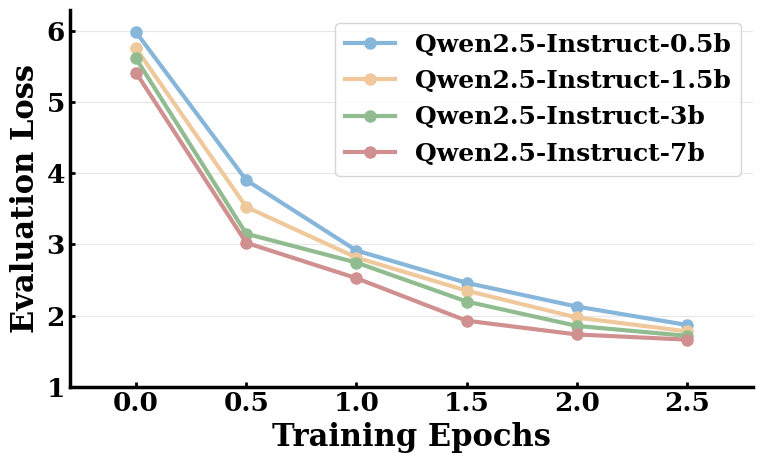
\includegraphics[width=\linewidth]{figures/scaling_eval_loss.png}
    \vspace{-16pt}                             % 细调下边距
    \caption{Evaluation loss vs.\ SFT training epoch}
    \label{fig:scaling_eval_loss}
\end{wrapfigure}
The comparison involves four systems:  
(1) GRU4Rec, trained and tested inside the \textit{Office} domain;  
(2) Qwen-Text, which represents user histories as plain sentences and predicts the next item by its title with no additional fine-tuning;  
(3) Qwen-SID, which encodes the same history with SID tokens and produces the next SID with no additional fine-tuning;  
(4) MiniOneRec-w/ RL-OOD, trained via GRPO on \textit{Industrial} only and evaluated on \textit{Office}, to evaluate its OOD (out-of-distribution) performance.

Table~\ref{tab:ood} reports the outcomes. Qwen-Text performs poorly, while Qwen-SID does noticeably better, indicating that a structured SID vocabulary is easier for an LLM to exploit. Although MiniOneRec-w/ RL-OOD falls short of the full MiniOneRec on in-domain scores, its reinforcement-only training grants excellent transfer, achieving competitive accuracy on the unseen catalog. Despite the substantial domain shift and possible semantic drift among SIDs, MiniOneRec successfully uncovers reusable interaction patterns, underscoring the framework’s promise for cross-domain recommendation.


% \subsection{Training and Inference Cost Comparison (RQ3)}

% To comprehensively evaluate the resource efficiency of MiniOneRec, we compare its training cost with that of SOTA LLM-based recommenders fine-tuned via SFT. Specifically, we report GPU-hours to provide a more granular view of the overall expenditure.
% We carry out the cost analysis on the industry scale Books dataset, as illustrated in Figure x. Although MiniOneRec still adopts a two-stage pipeline of SFT followed by RL, its inputs and outputs are encoded as SID sequences, whose token count is an order of magnitude smaller than the free form text used by previous LLM-based recommenders. On the Books corpus we reserve only a small held out split for the RL phase, so the additional computation remains marginal. Overall, MiniOneRec delivers marked performance gains without inflating the training budget and simultaneously preserves the multi-modal SID interface.
% Beyond training cost, we measure online efficiency by reporting average latency per recommendation request. Owing to its compact SID representation, MiniOneRec requires substantially fewer decoding steps during inference than other LLM-based baselines. As displayed in Figure x, MiniOneRec cuts inference latency by 70\%, while using the same GPU batch size. These results indicate that MiniOneRec is not only cost-effective during training but also practical for real-time serving scenarios.

% \subsection{Ablation Study (RQ3)}
\subsection{Ablation Study}

To validate the effectiveness of each component in the MiniOneRec framework, we compare it with the following alternative approaches. 

\subsubsection{Aligning Strategy}

% Please add the following required packages to your document preamble:
% \usepackage{multirow}
% \usepackage[table,xcdraw]{xcolor}
% Beamer presentation requires \usepackage{colortbl} instead of \usepackage[table,xcdraw]{xcolor}
\begin{table}[]
\caption{Performance of MiniOneRec and its variants on completely unseen recommendation domains} 
\label{tab:ood}
\resizebox{\textwidth}{!}{% 按比例缩放到页宽
% \begin{tabular}{clllllll}
\begin{tabular}{cccccccc}
\toprule
Dataset                           & Method                          & HR@3                           & NDCG@3                         & HR@5                           & NDCG@5                         & HR@10                          & NDCG@10                        \\ \hline
                                  & \cellcolor[HTML]{EFEFEF}GRU4Rec & \cellcolor[HTML]{EFEFEF}0.0629 & \cellcolor[HTML]{EFEFEF}0.0528 & \cellcolor[HTML]{EFEFEF}0.0789 & \cellcolor[HTML]{EFEFEF}0.0595 & \cellcolor[HTML]{EFEFEF}0.1019 & \cellcolor[HTML]{EFEFEF}0.0669 \\
                                  & Qwen-Text                       & 0.0031                         & 0.0021                         & 0.0044                         & 0.0026                         & 0.0057                         & 0.0030                         \\
                                  & Qwen-SID                        & 0.0300                         & 0.0214                         & 0.0456                         & 0.0282                         & 0.0733                         & 0.0373                         \\
\multirow{-4}{*}{\textbf{Office}} & \cellcolor[HTML]{ECF4FF}MiniOneRec-w/ RL-OOD              & \cellcolor[HTML]{ECF4FF}0.0553                         & \cellcolor[HTML]{ECF4FF}0.0433                         & \cellcolor[HTML]{ECF4FF}0.0691                         & \cellcolor[HTML]{ECF4FF}0.0489                         & \cellcolor[HTML]{ECF4FF}0.0892                         & \cellcolor[HTML]{ECF4FF}0.0553                         \\ \hline
\end{tabular}
}
\end{table}

To isolate the impact of each component, we compare the full MiniOneRec with three pared-down variants.  
(1) \textsc{MiniOneRec}--\textsc{w/o~Align}: removes any language–SID alignment and treats recommendation purely as a SID-to-SID task.  
(2) \textsc{MiniOneRec}--\textsc{w/~SFTAlign}: keeps the alignment objective during SFT stage only, while RL uses SID data alone.  
(3) \textsc{MiniOneRec}--\textsc{w/~RLAlign}: SFT relies solely on SID supervision, and the alignment tasks are introduced later in the RL stage.

Figure~\ref{fig:ab1} summarizes the findings. The complete MiniOneRec, which maintains alignment throughout the whole pipeline, delivers the highest scores on every metric. The \textsc{MiniOneRec}--\textsc{w/o~Align} performs worst, indicating that grounding SID generation in world knowledge is essential.

\subsubsection{Sampling Strategy}

We study how different roll-out methods affect MiniOneRec by switching only the trajectory generator while keeping everything else fixed:  
(1) \textsc{MiniOneRec}--\textsc{Common} relies on a plain Top-$k$ decoder to produce exactly the required number of paths.  
(2) \textsc{MiniOneRec}--\textsc{Dynamic} follows our two-step sampler: it first draws one and a half times the budget, then retains as many unique items as possible for RL.  
The full model adopts beam search with width 16.

As plotted in Figure~\ref{fig:ab2}, the complete MiniOneRec delivers the highest accuracy while using roughly two-thirds of the samples needed by the dynamic variant, demonstrating that beam search is the most cost-efficient choice among the tested strategies.

\subsubsection{Reward Design}

Three variants are compared:
(1) \textsc{MiniOneRec}--\textsc{w/~ACC} that relies solely on a binary correctness signal;  
(2) \textsc{MiniOneRec}--\textsc{w/~Collaborative} that replaces the ranking term with logits taken from a frozen SASRec model so as to supply collaborative cues;  

As shown in the Figure \ref{fig:ab3}, the full MiniOneRec achieves the best overall performance. To be noticed, injecting the collaborative reward information into the RL process instead led to significant degradation. We hypothesize that, this stems from reward hacking: as recommendation accuracy declines, the reward continues to increase, revealing a misalignment between this collaborative reward signal and the true objective.

\begin{figure*}[t]
  \centering
  \begin{subfigure}[t]{0.28\textwidth}
    \centering
    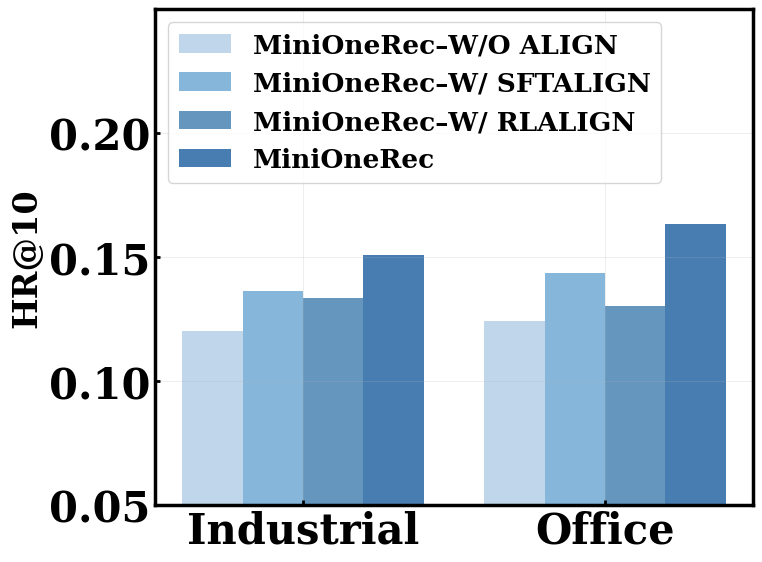
\includegraphics[width=\textwidth]{figures/ab1.png}
    \caption{Aligning Strategy.}
    \label{fig:ab1}
\end{subfigure}\hspace{2mm}
\begin{subfigure}[t]{0.28\textwidth}
    \centering
        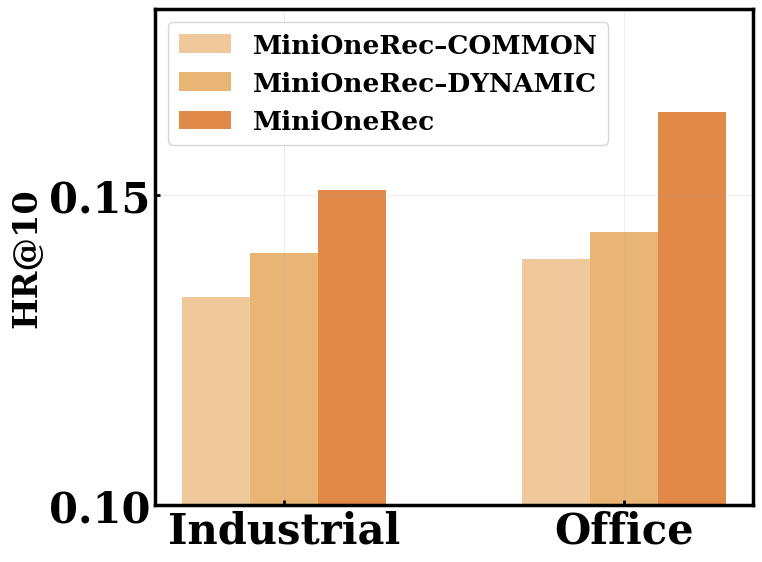
\includegraphics[width=\textwidth]{figures/ab2.png}
    \caption{Sampling Strategy.}
    \label{fig:ab2}
\end{subfigure}
\centering
  \begin{subfigure}[t]{0.28\textwidth}
    \centering
    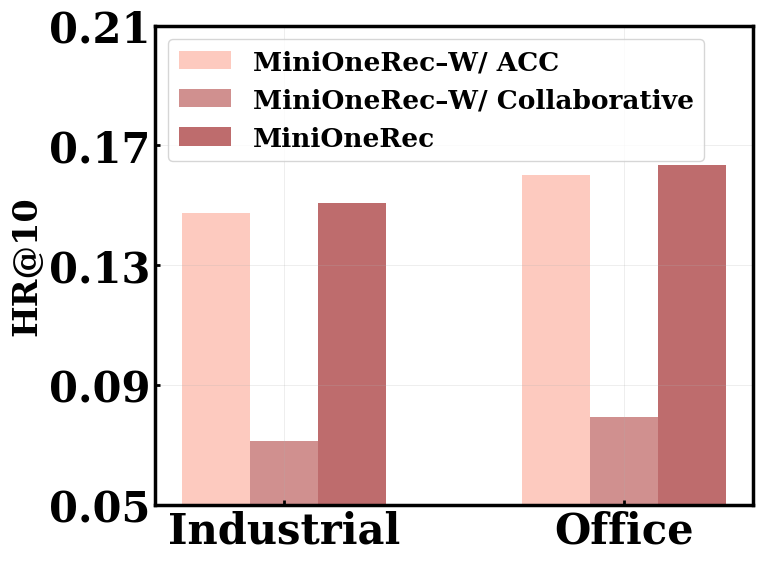
\includegraphics[width=\textwidth]{figures/ab3.png}
    \caption{Reward Design.}
    \label{fig:ab3}
\end{subfigure}\hspace{2mm}
  \caption{Study on the effectiveness of MiniOneRec’s individual components.
Figure \ref{fig:ab1} examines model performance under different alignment strategies;
Figure \ref{fig:ab2} investigates various sampling strategies;
Figure \ref{fig:ab3} evaluates the impact of alternative reward designs.}
  \label{fig:ablation}
    \vspace{-10pt}
\end{figure*}



% Please add the following required packages to your document preamble:
% \usepackage{multirow}
\begin{table}[]
\caption{Performance of MiniOneRec initialized with pre-trained weights versus random initialization across two domains} 
\label{tab:pretrain-impact}
\resizebox{\textwidth}{!}{% 按比例缩放到页宽
\begin{tabular}{clllllll}
\toprule
\multicolumn{1}{l}{Datesets}          & Methods            & HR@3            & NDCG@3          & HR@5            & NDCG@5          & HR@10           & NDCG@10         \\ \midrule
\multirow{2}{*}{\textbf{Industrial}} & MiniOneRec-scratch & 0.0757          & 0.0672          & 0.0891          & 0.0726          & 0.1134          & 0.0804          \\
                                     & \cellcolor[HTML]{ECF4FF}\textbf{MiniOneRec}         & \cellcolor[HTML]{ECF4FF}\textbf{0.1125} & \cellcolor[HTML]{ECF4FF}\textbf{0.0988} & \cellcolor[HTML]{ECF4FF}\textbf{0.1259} & \cellcolor[HTML]{ECF4FF}\textbf{0.1046} & \cellcolor[HTML]{ECF4FF}\textbf{0.1546} & \cellcolor[HTML]{ECF4FF}\textbf{0.1139} \\ \midrule
\multirow{2}{*}{\textbf{Office}}     & MiniOneRec-scratch & 0.0959          & 0.0855          & 0.1057          & 0.0896          & 0.1196          & 0.0941          \\
                                     & \cellcolor[HTML]{ECF4FF}\textbf{MiniOneRec}         & \cellcolor[HTML]{ECF4FF}\textbf{0.1217} & \cellcolor[HTML]{ECF4FF}\textbf{0.1088} & \cellcolor[HTML]{ECF4FF}\textbf{0.1420} & \cellcolor[HTML]{ECF4FF}\textbf{0.1172} & \cellcolor[HTML]{ECF4FF}\textbf{0.1634} & \cellcolor[HTML]{ECF4FF}\textbf{0.1242} \\ \bottomrule
\end{tabular}
}
\end{table}


\subsection{Pre-trained LLM Impact}
\label{llmmatter}
To isolate the impact of pre-trained LLMs on generative recommendation, we instantiate two variants of MiniOneRec: one initialized from a general-purpose pre-trained LLM and the other trained from scratch with random weights. As shown in Table \ref{tab:pretrain-impact}, Experiments on two benchmark datasets reveal a consistent pattern: the model that starts from pre-trained weights significantly outperforms its randomly initialized counterpart. We conjecture that (i) the general reasoning ability acquired during large-scale language pre-training allows the model to cast the next-SID prediction task as a problem of pattern discovery, as discussed in Section~\ref{subsec: Transferability}, and (ii) the factual knowledge already encoded in the LLM offers a head start in understanding the real-world semantics behind each SID, part of which can be transferred to the recommendation domain.